\subsection{Точные формулы для двухатомной системы}

Рассмотрим вектор, соединяющий центры атомов. Обозначим $\mf{r}$ его координаты в лабораторной системе координат, $\mf{R}$ -- в молекулярной системе координат. Производные $\mf{r}$ и $\mf{R}$ связаны при помощи матрицы эйлеровых углов $\bbS$ и угловой скорости $\mf{\Omega}$:
\begin{gather}
		\dot{\mf{r}} = \bbS^{-1} \lb \dot{\mf{R}} + \left[ \mf{\Omega} \times \mf{R} \right] \rb. \label{1} 
\end{gather}

Пусть атомы в молекулярной системе координат расположены на оси $Z$, в таком случае правая часть выражения \eqref{1} превращается в 
\begin{gather}
\dot{\mf{r}} = \bbS^{-1} \left\{
\begin{bmatrix}
		0 \\
		0 \\
		\dot{R}
\end{bmatrix}
+
\begin{bmatrix}
		\Omega_y R \\
		- \Omega_x R \\
		0
\end{bmatrix}
\right\} \notag \\
\bbS \dot{\mf{r}} =
\begin{bmatrix}
\Omega_y R \\
- \Omega_x R \\
\dot{R}
\end{bmatrix}. \label{2}
\end{gather}

Лагранжиан в молекулярной системе координат имеет следующий вид:
\begin{gather}
\mL = \frac{1}{2} \mu \dot{R}^2 + \frac{1}{2} \mf{\Omega}^\top
\begin{bmatrix}
		\mu R^2 & 0 & 0 \\
		0 & \mu R^2 & 0 \\
		0 & 0 & 0
\end{bmatrix}
\mf{\Omega} \notag
\end{gather}

Используя теорему Донкина, находим связь гамильтоновых переменных $\mf{J}$ и $\mf{p} = \left[ p_R \right]$ с лагранжевыми переменными $\mf{\Omega}$ и $\mf{q} = \left[ R \right]$:
\begin{gather}
\begin{aligned}
\mf{J} &= \frac{\partial \mL}{\partial \mf{\Omega}} = \bbI \, \mf{\Omega} \\
\mf{p} &= \frac{\partial \mL}{\partial \dot{\mf{q}}} = \bba \, \dot{\mf{q}}
\end{aligned}
\quad \implies \quad
\begin{aligned}
		J_x &= \mu R^2 \, \Omega_x \\
		J_y &= \mu R^2 \, \Omega_y \\
		p_R &= \mu \dot{R}
\end{aligned} \label{3}
\end{gather}

Выкладка в приложении \ref{app1} показывает, что каждая компонента $\dot{\mf{r}}$ имеет нормальное распределение $\dot{\mf{r}} \sim \mathcal{N} \lb \mu = 0, \sigma^2 = \displaystyle \frac{kT}{\mu} \rb$. \par
``Экспериментально``  проверено, что действие равномерно распределенной матрицы поворота $\bbS$ на $\dot{\mf{r}}$ не приводит к изменению распределения $\dot{\mf{r}}$. Это интуитивно понятно, но строгого доказательства пока нет. Используем этот ``экспериментальный``  факт для получения точных распределений для переменных $J_x$, $J_y$ и $p_R$:
\begin{gather}
	\bbS \dot{\mf{r}} \sim \dot{\mf{r}} \sim
	\begin{bmatrix}
		\Omega_y R \\
		- \Omega_x R \\
		\dot{R}
	\end{bmatrix}
	\quad \implies \quad
	\begin{aligned}
			\Omega_x R &\sim \mN \lb 0, \frac{k T}{\mu} \rb \\
			\Omega_y R &\sim \mN \lb 0, \frac{k T}{\mu} \rb \\
			\dot{R} &\sim \mN \lb 0, \frac{k T}{\mu} \rb 
	\end{aligned} \quad \implies \quad  
	\begin{aligned}
			J_x &\sim \mu \, \Omega_x R^2 \sim \mN \lb 0, k T \mu R^2 \rb \\
			J_y &\sim \mu \, \Omega_y R^2 \sim \mN \lb 0, k T \mu R^2 \rb \\
			p_R &\sim \mu \dot{R} \sim \mN \lb 0, k T \mu \rb  
	\end{aligned} \notag 
\end{gather}

\begin{figure}[ht!]
		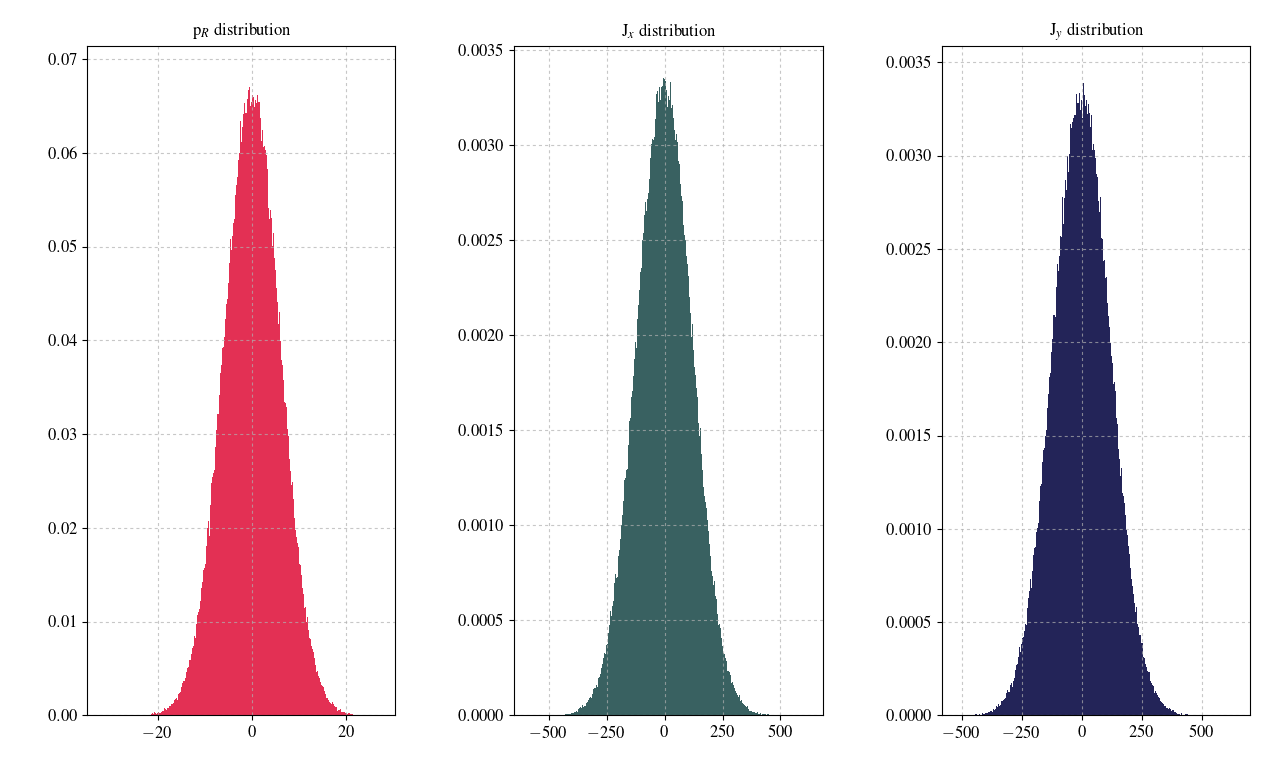
\includegraphics[width=\textwidth]{../pictures/diatomicsDistributions.png}
		\caption{Распределения переменных $p_R$, $J_x$, $J_y$ для двух атомов с массами $m_{Ar}$ и $m_{CO_2}$ при $T = 300 K$, 500.000 точек.}
\end{figure}

\begin{lstlisting}
#include <iostream>
#include <random>

using namespace std;

// boltzamnn constant 
const double BOLTZCONST = 1.38064e-23;
// dalton to kg 
const double DALTON = 1.660539e-27;
// atomic length unit to m 
const double ALU = 5.29177e-11;

// reduced mass of ar and co2 = m(ar) * m(co2) / (m(ar) + m(co2)) in kg
const double MU = 20.952 * DALTON;

// planck constant 
const double HBAR = 1.0545718e-34;

const double temperature = 300;

// distance between atoms 
const double RDIST = 20.0;

// a Mersenne Twister pseudo-random generator of 32-bit numbers with a state size of 19937 bits
static thread_local mt19937 generator;
 
double nextGaussian( const double &mean, const double &sigma )
{
    normal_distribution<double> d( mean, sigma );
    return d( generator ); 
} 

int main( int argc, char* argv[] )
{
	int n = atoi( argv[1] );

	for ( int i = 0; i < n; i++ )
	{
		double jx = nextGaussian( 0, RDIST * ALU * sqrt(BOLTZCONST * temperature * MU )) / HBAR;
		double jy = nextGaussian( 0, RDIST * ALU * sqrt(BOLTZCONST * temperature * MU )) / HBAR;
		double pR = nextGaussian( 0, sqrt(BOLTZCONST * temperature * MU)) / HBAR * ALU;

		cout << jx << "  " << jy << "  " << pR << endl;
	}

	return 0;
}
\end{lstlisting}

Пример программы на С++ для генерации значений $J_x$, $J_y$ и $p_R$ по точным распределениям.

